\section*{Einleitung}

\begin{frame}{Motivation: Anwendungsfall E-Commerce I}
    \begin{itemize}
        \item Ziel: Backend für internationales E-Commerce-System
        \item MVP: Bestellungen, Bezahlung und Versand
        \item Zukünftig viele Nutzer und hoher Traffic erwartet
        \item Geringes Kapital für Infrastruktur
        \item Rechtliche Regularien teilweise unklar, weil international
        \item Hohe Sicherheitsanforderungen
        \item Agiles Team von acht fähigen Entwicklern
        \item Geldgeber wollen erste Auslieferung in zwei Wochen
    \end{itemize}
\end{frame}

\begin{frame}{Motivation: Anwendungsfall E-Commerce II}
    \begin{figure}[!h]
        \centering
        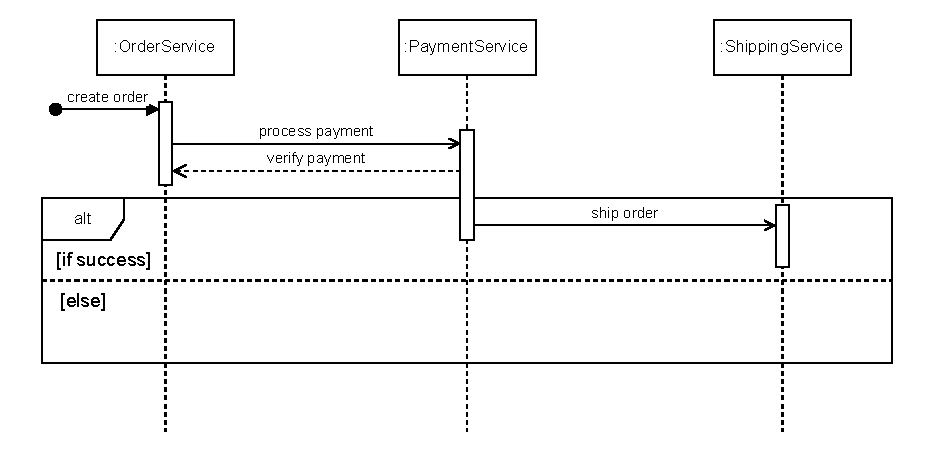
\includegraphics[scale=0.65]{imglib/einleitung/ecommerce.drawio}
        \caption{Sequenzdiagram zum Aufgeben einer Bestellung}
        \label{fig:ecommerce}
    \end{figure}
\end{frame}
